\documentclass[12pt]{article}

\usepackage{amsmath}
\usepackage{sbc-template}
\usepackage{graphicx,url}
\usepackage[brazil]{babel}   
\usepackage[utf8]{inputenc}  
     
\sloppy

\title{Análise da Correlação entre a Temperatura Global e o Preço Real do Café}

\author{Adriano Araújo D. Santos\inst{1}}

\address{Instituto de Ciências Exatas e Informática -- Pontifícia Universidade
\\ Católica de Minas Gerais (PUC Minas)
\\ R. Cláudio Manoel, 1162 -- Savassi - 30.140-100 -- Belo Horizonte -- MG -- Brasil
\email{adriano.domingos@sga.pucminas.br}
}

\begin{document} 

\maketitle

\begin{abstract}
This paper investigates the relationship between global temperature anomalies and coffee prices. The analysis considers the period from 1974 to 2024, the deviation from the mean historical global temperature and the price of coffee beans per kilogram in US dollars (USD). Presenting an overview of the dataset, sampling and cleaning procedures, exploratory statistical analysis, visualizations, and a critical interpretation of the results.
\end{abstract}

\begin{resumo} 
Este artigo investiga a relação entre anomalias de temperatura global e o preço do café. A análise abrange o período de 1974 a 2024, considerando o desvio em relação à média histórica da temperatura global e o preço do café por quilograma em dólares americanos (USD). Apresenta-se a descrição geral da base de dados, o processo de amostragem e de limpeza dos dados, análise exploratória com medidas estatísticas, visualizações e interpretação crítica dos resultados.
\end{resumo}

\section{Introdução} \label{sec:introduction}
O clima impacta diversas áreas, dentre as quais a agricultura se destaca. Por isso, surge a questão sobre o efeito das anomalias de temperatura na produção de café.

As mudanças climáticas tornaram-se um dos principais desafios globais nas últimas décadas, afetando diretamente vários setores econômicos e sociais. A agricultura é especialmente sensível, pois o clima influi fortemente no desenvolvimento e na produtividade das culturas \cite{pinto:2004}.

Diante da crescente preocupação com o aquecimento global e suas implicações, torna-se essencial compreender como as elevadas temperaturas ao longo dos anos têm afetado a produção de café. Nesse contexto, uma análise que relacione as anomalias de temperatura global com a evolução dos preços do café ajustados pela inflação revela-se relevante.

Este estudo propõe-se a investigar essa possível relação no período de 1974 a 2024, utilizando ferramentas de análise de dados, estatística descritiva e visualização gráfica.

\section{Justificativa}
A escolha deste tema deve-se ao pronunciado aumento dos preços do café ocorrido em 2025 \cite{cnnbrasil:2025}, levantando questionamentos sobre os fatores de longo prazo que influenciam essa commodity. Em especial, verifica-se se as tendências de aquecimento global, medidas por anomalias de temperatura, podem explicar parte da variação histórica dos preços do café ajustados pela inflação.

\section{Identificação da Base de Dados}

\subsection{Origem e Descrição Geral}
Os dados utilizados foram obtidos manualmente em três fontes distintas: o histórico de preços do café da plataforma Macrotrends \cite{macrotrends}, as anomalias globais de temperatura registradas pelo GISS da NASA \cite{gistemp} e os valores do Índice de Preços ao Consumidor (CPI) do U.S. Bureau of Labor Statistics \cite{usbls}. As informações foram extraídas em formato tabular e unificadas em uma planilha no Google Sheets.

A base final possui frequência mensal, cobrindo de janeiro de 1974 a dezembro de 2024, totalizando 612 observações. Cada entrada corresponde a um mês específico e contém o preço do café, a anomalia de temperatura global e o CPI do período.

\subsection{Dicionário de Dados}
\begin{table}[ht]
\centering
\caption{Dicionário de dados utilizados}
\begin{tabular}{l l p{8cm}}
\hline
\textbf{Campo} & \textbf{Tipo} & \textbf{Descrição} \\
\hline
Ano & Número Inteiro & Ano da observação (1974-2024) \\

Mês & Número Inteiro & Mês da observação (1-12) \\

Anomalia (°C) & Número Real & Anomalia de temperatura global em °C em relação à média histórica \\

Anomalia (\%) & Número Real & Variação percentual da anomalia de temperatura em relação à média histórica \\

Preço Nominal (USD/lb) & Número Real & Preço nominal do café por libra em dólares americanos \\

CPI & Número Real & Índice de Preços ao Consumidor do mês correspondente \\

Preço Ajustado (USD/lb) & Número Real & Preço do café por libra, ajustado pela inflação \\

Preço Ajustado (USD/kg) & Número Real & Preço do café por quilograma, ajustado pela inflação \\

Preço Ajustado (\%) & Número Real & Preço do café em percentual em relação ao maior valor do período \\
\hline
\end{tabular}
\end{table}

\subsection{Amostra e Limpeza de Dados}
A integração das bases foi realizada manualmente, transpondo-se as tabelas de temperatura e CPI e concatenando-as com os registros de preço. O tratamento e a padronização ocorreram no Google Sheets, com uso de fórmulas para ajustes monetários e de unidades. Os preços foram convertidos de libra para quilograma (multiplicação por 0,453592) e ajustados pela inflação conforme a fórmula:

\begin{center}
$\displaystyle \text{Valor~Corrigido} = \frac{\text{Valor~Nominal}}{\text{CPI~do~Mês}} \times \text{CPI~de~Dezembro~de~2024}$
\end{center}

As anomalias de temperatura já estavam em graus Celsius, e foi padronizado o uso de ponto decimal e vírgula conforme o padrão brasileiro. Não foram encontrados valores ausentes ou inconsistentes nas bases utilizadas, sendo necessária apenas a padronização das casas decimais e o alinhamento das datas.

\section{Definição do Problema}
\subsection{Pergunta de Pesquisa}
\textit{Como as anomalias de temperatura global influenciaram os preços do café (ajustados pela inflação) entre 1974 e 2024?}

\subsection{Variáveis Utilizadas}
Para responder à pergunta, empregaram-se duas variáveis principais: a anomalia de temperatura global e o preço do café, ambas expressas em percentuais para facilitar a comparação.

As variáveis consideradas foram:

\begin{itemize}
  \item \textbf{Anomalia (\%)}: percentual de alteração da temperatura global em relação à média histórica, evidenciando desvios e tendências.
  \item \textbf{Preço Ajustado (\%)}: preço do café ajustado pela inflação, relativo ao maior valor do período, permitindo comparação da evolução sem efeito de escala monetária.
\end{itemize}

Ambas têm frequência mensal. A adoção de percentuais simplifica a interpretação da relação, e o uso de USD/kg ajustado pela inflação atende ao padrão científico, facilitando comparações futuras.

\section{Análise Exploratória de Dados}

Nesta seção, apresentam-se medidas estatísticas calculadas para anomalias de temperatura e preços ajustados do café no período de 1974 a 2024. A análise por década permite identificar padrões de longo prazo e mudanças comportamentais.

\subsection{Correlação entre Variáveis}
Um dos objetivos centrais desta análise foi investigar a existência de uma relação estatística linear entre a anomalia de temperatura global e o preço do café ao longo do tempo. Para isso, calculou-se o coeficiente de correlação de Pearson entre as variáveis \textbf{Anomalia (\%)} e \textbf{Preço Ajustado (\%)}.

O valor obtido foi \textbf{-0,5328}, indicando uma correlação negativa moderada. Isso sugere que, entre 1974 e 2024, anos com maiores anomalias de temperatura tenderam a estar associados a reduções relativas nos preços ajustados do café. Essa relação pode estar associada a fatores como adaptação agrícola, variação de produtividade, deslocamento de zonas de cultivo e transformações estruturais na cadeia de produção.

Análises segmentadas por décadas revelaram variações na intensidade da correlação, com valores mais fracos em períodos intermediários -- por exemplo, \textbf{-0,3071} entre 1984 e 1993 -- e intensificação na série completa, o que pode refletir uma tendência de longo prazo possivelmente relacionada aos efeitos cumulativos do aquecimento global.

Cabe destacar que a correlação de Pearson não implica causalidade, e os preços do café são influenciados por múltiplos fatores externos, incluindo políticas agrícolas, dinâmica de oferta e demanda, flutuações cambiais, logística internacional e eventos geopolíticos. Uma interpretação mais abrangente exige uma abordagem multidisciplinar que integre variáveis econômicas, climáticas e tecnológicas.

\subsection{Medidas de Tendência Central e Dispersão}
Foram calculadas as seguintes medidas estatísticas para as variáveis \textit{Anomalia (°C)}, \textit{Anomalia (\%)}, \textit{Preço Ajustado (USD/kg)} e \textit{Preço Ajustado (\%)}:

\begin{itemize}
  \item \textbf{Média}, \textbf{Mediana}: indicam a tendência central das variáveis em cada década.
  \item \textbf{Desvio Padrão}: expressa a variabilidade dos dados em torno da média.
  \item \textbf{Percentis 25\%, 50\% e 75\%}: fornecem informações sobre a distribuição dos valores em cada período.
\end{itemize}

Ao longo das décadas, observou-se um aumento progressivo na média da anomalia de temperatura, com destaque para o período entre 2014 e 2024, que apresentou média de 0,9672°C e mediana de 0,9200°C. Em contrapartida, o preço ajustado do café em USD/kg apresentou tendência de queda, com média passando de 2,8010 na década de 1974–1983 para 0,8267 na década de 2014–2024.

\subsection{Outros Padrões Observados}
A análise exploratória revelou que o período de 1974 a 1983 se destacou por um aumento expressivo no preço do café ajustado, com média de 2,8010 USD/kg, muito superior às décadas seguintes. Esse pico pode estar relacionado a choques climáticos ou econômicos específicos da época.

O uso de percentuais para anomalia e preço ajustado auxiliou na comparação direta das variações relativas de ambas as variáveis ao longo do tempo. As análises evidenciam uma tendência de aumento contínuo das anomalias térmicas e um comportamento decrescente nos preços reais do café.

\section{Visualização de Dados}
Nesta seção, seguem três tipos principais de gráficos: evolução temporal, relação entre variáveis e distribuição por períodos. Os gráficos baseiam-se em séries mensais e estatísticas agregadas por década.

\subsection{Evolução Temporal}

\begin{figure}[ht]
\centering
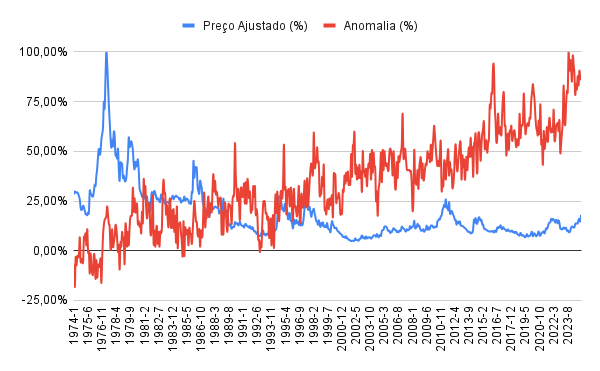
\includegraphics[width=1\textwidth]{evolucao-temporal.png}
\caption{Evolução temporal da Anomalia de Temperatura e do Preço Ajustado do Café (\%).}
\label{fig:evolucao}
\end{figure}

Na \textbf{Figura \ref{fig:evolucao}}, é possível observar que ao longo dos 50 anos de observação, as anomalias de temperatura apresentaram tendência crescente, enquanto os preços ajustados do café, em termos relativos, apresentaram queda contínua ao longo do período.

Após o período inicial, observa-se que o preço relativo do café teve uma certa estabilidade, principalmente na última década observada. A divergência entre as duas curvas ao longo das décadas reforça a hipótese de uma possível relação inversa entre aumento da temperatura e redução do preço do café ajustado.

Outro aspecto notável é que, enquanto a curva de anomalia mostra uma tendência ascendente contínua, a curva de preços ajustados estabiliza em patamares baixos, sugerindo que o mercado de café pode estar sofrendo pressões prolongadas, tanto climáticas quanto estruturais. Isso pode incluir fatores como avanço tecnológico, mudança nos padrões de consumo, aumento da concorrência internacional e adaptação dos produtores às novas condições ambientais.

\subsection{Dispersão entre Temperatura e Preço}
A \textbf{Figura \ref{fig:dispersao}} mostra a relação entre a Anomalia e o Preço Ajustado para todo o período analisado. Como esperado pela análise estatística, é possível observar uma tendência geral de correlação negativa, ainda que com dispersão relevante.

A linha de tendência adicionada ao gráfico reforça essa correlação negativa, destacando que conforme a anomalia de temperatura aumenta, os preços ajustados do café tendem a diminuir. A inclinação da linha de regressão revela uma razão média de queda de aproximadamente \textbf{0,284 USD/kg} para cada grau Celsius de aumento na anomalia de temperatura.

Além disso, observa-se que os preços mais altos estão concentrados em valores de anomalia entre 0°C e 0,25°C, onde pontos acima de 4,00 USD/kg são frequentes. Por outro lado, quando as anomalias ultrapassam 1°C, os preços ajustados ficam majoritariamente abaixo de 1,00 USD/kg, indicando uma possível diminuição de preço associada ao aquecimento global.

\begin{figure}[ht]
\centering
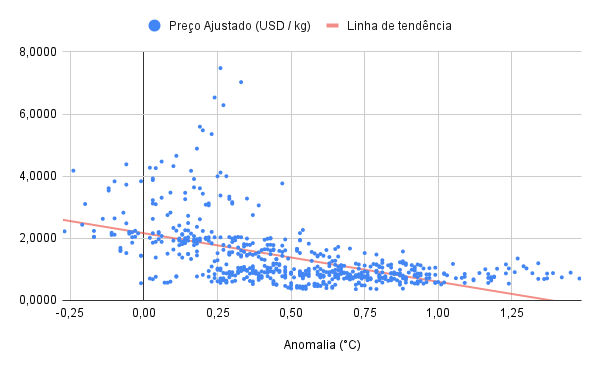
\includegraphics[width=1\textwidth]{dispersao.png}
\caption{Dispersão entre Anomalia de Temperatura e Preço Ajustado do Café.}
\label{fig:dispersao}
\end{figure}

\subsection{Distribuição por Década}
A análise por década revela importantes diferenças na distribuição dos preços ajustados do café. A \textbf{Figura \ref{fig:periodos}} apresenta as principais estatísticas descritivas para cada período, incluindo média, desvio padrão, percentis e mediana.

Nota-se que o período entre 1974 e 1983 apresenta valores significativamente mais altos para todas as estatísticas, o que corrobora a presença de um aumento brusco no preço do café nessa década. A média de aproximadamente 2,80 USD/kg e o percentil 75\% acima de 3,48 USD/kg evidenciam um comportamento atípico em comparação às décadas seguintes.

Já a partir da década de 1990, observa-se uma estabilização e posterior queda dos preços. A última década (2014–2024) apresenta a menor média registrada, com valores concentrados entre 0,69 e 0,99 USD/kg. Esse comportamento pode indicar uma adaptação do mercado às novas condições climáticas ou transformações estruturais na produção e comercialização do café.

\begin{figure}[ht]
\centering
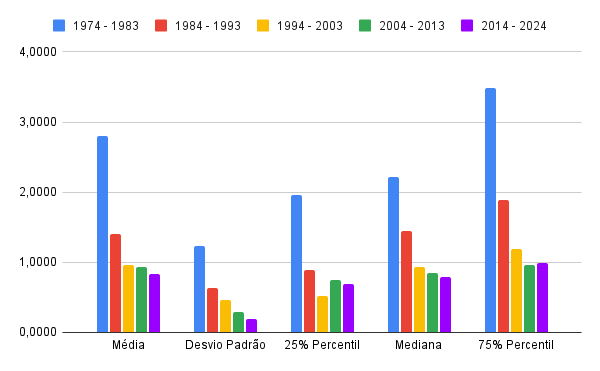
\includegraphics[width=0.9\textwidth]{periodos.png}
\caption{Distribuição das variáveis por década (1974–2024).}
\label{fig:periodos}
\end{figure}

\section{Conclusão}

\subsection{Análise Crítica e Interpretação dos Resultados}
A análise exploratória e as visualizações evidenciaram uma correlação moderadamente negativa \textbf{(–0,5328)} entre as anomalias de temperatura global e o preço ajustado do café, sugerindo que, em média, cada aumento de \textbf{1 °C} na anomalia está associado a uma redução de cerca de \textbf{0,284 USD/kg} no preço real do grão. 

Observou-se também que, grandes picos de preço ocorreram na década de 1974–1983, provavelmente impulsionados por fatores externos ainda não modelados neste estudo. E ocorreu uma tendência de queda nos preços ajustados a partir dos anos 1990, coincidindo com o aquecimento contínuo, reforçando o impacto das mudanças climáticas sobre o mercado cafeeiro.

\subsection{Limitações do Estudo}
Este estudo apresentou algumas limitações que devem ser consideradas:

\begin{itemize}  
  \item \textbf{Fatores Externos Não Modelados:} Políticas comerciais, custos de transporte, subsídios agrícolas e eventos geopolíticos podem afetar fortemente os preços, mas não foram incorporados.
  \item \textbf{Granularidade Global:} A análise usa dados globais mensais, sem discriminar por regiões produtoras, o que pode mascarar variações locais.
  \item \textbf{Horizonte Temporal e Estrutural:} Embora cubra 50 anos, mudanças tecnológicas no cultivo e na logística de mercado não foram modeladas.
  \item \textbf{Abordagem Simples de Modelagem:} Foram usadas apenas correlação e regressão linear; modelos causais ou dinâmicos poderiam oferecer maior profundidade.
\end{itemize}

\subsection{Sugestões para Trabalhos Futuros}
Para aprofundar o entendimento dos impactos climáticos sobre os preços do café, outros pontos que poderiam ser desenvolvidos seriam:

\begin{itemize}
  \item \textbf{Análise Regionalizada:} Estudar separadamente as principais regiões produtoras (Brasil, Colômbia, Vietnã) para capturar efeitos locais do clima.
  \item \textbf{Modelagem Avançada:} Aplicar séries temporais multivariadas e testes de causalidade de Granger para explorar relações dinâmicas.
  \item \textbf{Inclusão de Variáveis Macroeconômicas:} Integrar taxas de câmbio, custos de insumos e políticas de subsídio para isolar o efeito climático.
  \item \textbf{Resiliência da Cadeia de Suprimentos:} Avaliar estratégias de adaptação, como variedades resistentes ao calor e instrumentos financeiros de hedge.
\end{itemize}

\bibliographystyle{sbc}
\bibliography{sbc-template}

\end{document}
